% res_leave.tex -- Results 4.2: leaving the team (RQ2). 17 Oct (v3_full): sim_detach.tex and skel_leave.tex merged.
% Rig: the 7-8 Oct releases (T8a/T8b filled 12 Oct from docs/analysis/p6_offline_2026-10-12.md after the reviewer;
% L labels mapped in docs/figures/PROVENANCE.md: L1 r0012, L2 r0013, L3a/L3b r200006, L4 r302_3, L5 r303_4, L6 r304_3,
% L7 r305; L8/L9 the hover and circle releases of the next rig day); L10 RIG-1014-t5_2, L11 RIG-1015-a2_2 (registry
% rows; not scored on the frozen metric). Twin, detach freeze tree (week5 4b3560e flight code, lab batch 15): Tier A
% rev 3 (T3, T8, T9, K1, T15; reviewer SUPPORTED WITH CORRECTIONS 16 Oct), Tier B (B1-B3, B5 confirmed; B4 falsified as
% written), W4/W5 F1 and departed P1-P4 (departed_disarm_alone), drop and land v3 (D1, D4; SUPPORTED). Must-not-say
% lists of all four cards honoured (see each card). T10 from tools/thesis_freeze_tables.py; F10b and F12 from
% tools/thesis_lever_figures.py. fig:detach is the 17 Oct re-render of R1887 (A1 r1).

\subsection{Leaving the team}
\label{sec:res_leave}

This section answers RQ2: when a carrier leaves in flight, what sets the ring's transient, and what keeps the ring
from being lost? The rig gives the record of every release, commanded or not. The twin gives the levers, each a
one-variable pair flown on one code tree against a named baseline and scored by the resolution rule frozen before
the runs (Section~\ref{sec:metrics}); each pair is labelled a replication or a new prediction. The primary metric is
the tilt rise $\Delta\theta$; the 30$^\circ$ drop rule is the safety line.

\subsubsection{Every release on the rig}
\label{sec:res_detach_rig}

Table~\ref{tab:T8b} holds every release on the rig, with the uncommanded ones (their conditions in
Table~\ref{tab:T8a} and a drawing in Figure~\ref{fig:F10}, Appendix~\ref{sec:app_secondary}). Six releases were commanded. On 7 October, with the rods planned at 45$^\circ$ and
the trackers on the planner's pull, an announced release was carried through (L1) and a second one lost the ring
when two survivors' magnets let go after it (L2). On 8 October, with the rods at 60$^\circ$ and the measured pull, all
four releases were carried through, announced and unannounced, in hover and on the circle, with a 120$^\circ$ or a
150$^\circ$ gap left (L4--L7; Figure~\ref{fig:rig_detach}, Appendix~\ref{sec:app_secondary}). Over the five releases carried through the tilt rise was
5.3--16.9$^\circ$, and the planner found the three unannounced ones from the stretched rod 0.33--0.42\,s after the
magnet was switched off, the magnet's own release time included. On the circle (Figure~\ref{fig:rig_circle_detach})
the planner held the path for 1.5\,s from the detection while the three survivors took up the freed UAV's share, then
carried the ring on round it, while the freed UAV cleared the circle and began its own landing 6.1\,s after the
release. The hover and circle releases on the current defaults (L8, L9) wait for the next rig day.



\begin{table}[htbp]
  \centering
  \footnotesize
  \caption[The rig release record: outcomes]{The hardware release record, outcomes (T8b), against the twin's range for
  the same configuration. $\Delta\theta$: the tilt-vector departure from the 5\,s pre-event mean, to LAND
  (Section~\ref{sec:metrics}); peak: the largest absolute tilt over the same window; dip: the ring's lowest height
  against its pre-event mean; back in band: scored only when LAND came 10\,s or more after the event (n/s otherwise);
  landing lean: the largest survivor tilt 1.2\,s after the ring touched down; survivor step: the largest planned
  tension step handed to a survivor in the first second of the resized plan; twin: the pair's $\Delta\theta$ range cut
  at the rig flight's hold. $\geq$: the log ends at the fleet's latch with the tilt still rising, a lower bound. L3a
  and L3b are timed from the slip onset in the bag; L3b's pre-window contains L3a. L10, L11: from the flight logs, not
  yet on the frozen metric. [L8 and L9: the next rig day, against the bands of Section~\ref{sec:ledger}.]}
  \label{tab:T8b}
  \begin{tabularx}{\textwidth}{lYYYYYYYY}
    \toprule
    Event & Detection (s) & $\Delta\theta$ ($^\circ$) & Peak ($^\circ$) & Dip (cm) & Back in band (s) & Landing lean ($^\circ$)
      & Survivor step (N) & Twin, $n$ \\
    \midrule
    L1 & -- & 6.1 & 5.5 & none & n/s & 3.5 & +1.2 & -- \\ % r0012: dtheta exceeds the peak (a 1.5 deg pre-mean, the tilt swung 177 deg away from it); the 5.5 came 0.1 s before LAND, the first second peaked at 4.6; the ring rose 15 cm, no dip; one twin run (R1093) exists, not on the frozen metric
    L2 & -- & $\geq$68.3 & $\geq$68.6 & 21.7 & -- & capsized & +2.8 & -- \\ % r0013: the log ends at the fleet abort 0.47 s after the release with the tilt still rising (the planner read 89 deg at +0.61 s); P6's step in the first second; the registry's first resized row reads +1.8; one twin run on these settings (R1125, no capsize), not on the frozen metric
    L3a & -- & 30.9 & 30.6 & 12.5 & -- & -- & none (3.0 per rod) & -- \\ % r200006 slip 1: timed from the slip onset in the bag, not a frozen event time; pre-window flagged (the orbit's speed ramp); operator LAND 0.59 s after; the ring recovered
    L3b & -- & $\geq$63.2 & $\geq$65.5 & 68.1 & -- & capsized & none & -- \\ % r200006 slip 2: the log ends at the fleet abort 0.43 s after; the pre-window holds slip 1 (sigma_pre 8.6 deg)
    L4 & -- & 11.2 & 15.4 & 6.9 & n/s & 2.5 & +1.2 & 6.0--7.1, 2 \\ % r302_3; twin R1207, R1212 cut at the rig's 6.6 s hold
    L5 & 0.42 & 5.3 & 6.5 & 3.1 & n/s & 3.0 & +1.2 & 6.0--6.4, 2 \\ % r303_4; twin R1712/R1713 (int_mode model, Wesley 16 Oct (4); the rig flew reference) read 6.04-6.34; R1140/R1145 (reference) 6.00/6.44
    L6 & 0.33 & 16.9 & 17.8 & 5.3 & n/s & 3.3 & +1.7 & 14.6--17.4, 2 \\ % r304_3; twin R1206, R1211 (7.7 s)
    L7 & 0.34 & 8.0 & 8.1 & 3.7 & 3.9 & 4.0 & +1.1 & 4.0--5.4, 2 \\ % r305; twin R1208, R1213 (14.0 s); back in band with a half-width of 4.7 deg (2 sigma_pre), nine times the twin's 0.5 deg: the times do not compare
    L8 & [\dots] & [\dots] & [\dots] & [\dots] & [\dots] & [\dots] & [\dots] & band 1.75--14.51 \\
    L9 & [\dots] & [\dots] & [\dots] & [\dots] & [\dots] & [\dots] & [\dots] & band 1.00--13.20 \\
    L10 & -- & [\dots] & 70--81, capsized & -- & -- & -- & -- & -- \\ % RIG-1014-t5_2: ring 70-81 deg; envelope fault, fleet disarm from ~1 m
    L11 & -- & [\dots] & 36.8, dropped & -- & -- & -- & -- & -- \\ % RIG-1015-a2_2: ring tilt 36.8 deg -> drop rule
    \bottomrule
  \end{tabularx}
\end{table}
% L5's twin column: Wesley 16 Oct (4) switched it to R1712/R1713, which flew the model integral where the rig flew the
% reference integral; the numbers agree (6.04-6.34 against 6.00-6.44), and this note says so.
% Layouts in today's plate numbering (clockwise from +x; 30/90/150/270 deg counter-clockwise = plates 11/9/7/3).





\begin{figure}[htbp]
\centering
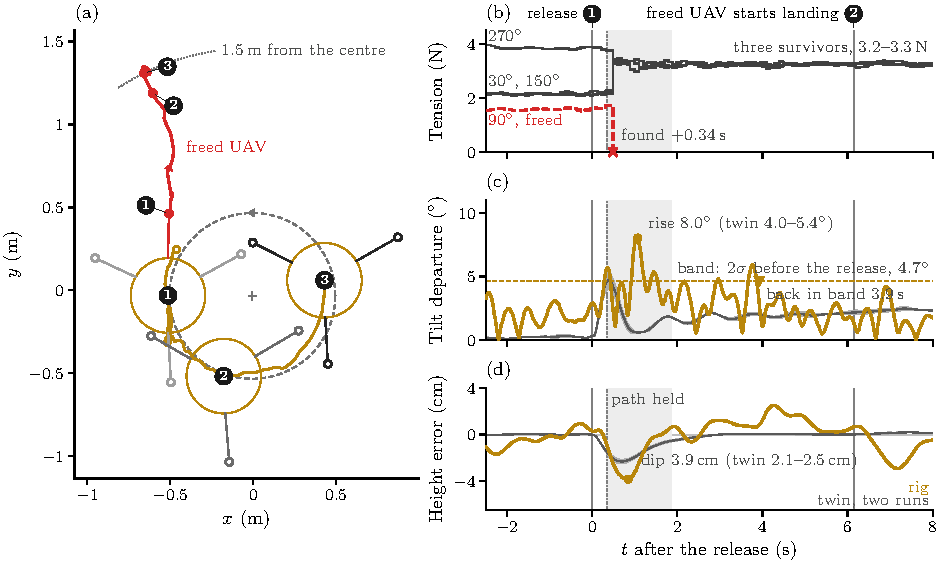
\includegraphics[width=\textwidth]{Images/rig_circle_detach.pdf}
\caption[Unannounced release during the circle on the rig]{An unannounced release during the circle on the rig, 8
October: four UAVs on plates 3, 7, 9 and 11 carry the ring round a circle of radius 0.5\,m at 0.125\,m/s, and the magnet
on plate 9 is switched off without telling the planner (the panels print counter-clockwise azimuths: 30$^\circ$ is plate
11, 90$^\circ$ plate 9, 150$^\circ$ plate 7, 270$^\circ$ plate 3). (a) Plan view: the circle, the ring's centre and the
fleet at the release (1), when the freed UAV starts its own landing 6.1\,s later (2), and at LAND, 14.0\,s after the
release (3). (b) The planner's tension per UAV: the freed UAV's (dashed) stays in the plan until the planner finds the
release from its stretched rod 0.34\,s after it; the three survivors then share the ring at 3.2--3.3\,N each; grey band:
the path held for 1.5\,s. (c) The ring's tilt departure and (d) its height error, the rig (gold, one run) against the
twin flying the same configuration (grey, two runs): the rig's tilt rise is 8.0$^\circ$ against the twin's
4.0--5.4$^\circ$, and its lowest height error 3.9\,cm against 2.1--2.5\,cm.}
\label{fig:rig_circle_detach}
\end{figure}

Against the rig's own rocking with no event, L4 and L6 stand clear on raw $\Delta\theta$, L5 does too once scaled by
its own rocking, and L1 and L7 do not (Appendix~\ref{sec:app_secondary}).

\paragraph{How the ring was lost.} Every ring lost on the rig began with a magnet letting go with no command
(Figure~\ref{fig:F11}). In L2 the planner raised the largest survivor's tension, within the first second after the
resize, by up to 2.75\,N (+1.8\,N at its first solve), against the 1.61\,N the statics of that layout ask for, and a
survivor's magnet let go 0.17\,s after the release at 2.6$^\circ$ of tilt; on 8 October, on the measured pull, the same layout's step was 1.74\,N and the ring recovered. In L3 a magnet let go
in a steady circle at 0.9$^\circ$ of tilt with every rod at 3.0\,N. Two more let go after the rods were planned at
60$^\circ$, both in the attach flights with three carriers. On 14 October (L10) the three-carrier lift ran with the carriers' commands at 42--44\,Hz
instead of 50 under the combined attach stack, the ring bobbed at about 1\,Hz with a growing amplitude, every pose and
command stream froze for 0.25\,s, and half a second later one carrier's magnet let go (whether the slowed loops or the
freeze caused it is open); with two carriers left and the drop rule then
off in that mode, the ring capsized and the fleet was disarmed about 1\,m up. The drop rule has been on in every mode
since. On 15 October (L11) a carrier let go of plate 7 in a steady hover with nothing touching it and its pack at
21.9\,V; the ring tilted to 36.8$^\circ$, the drop rule switched every magnet off, and every carrier landed and was
disarmed alone. Whether heat or a low pack weakened that hold is open: nothing records the coils' current or
temperature.

\begin{figure}[htbp]
\centering
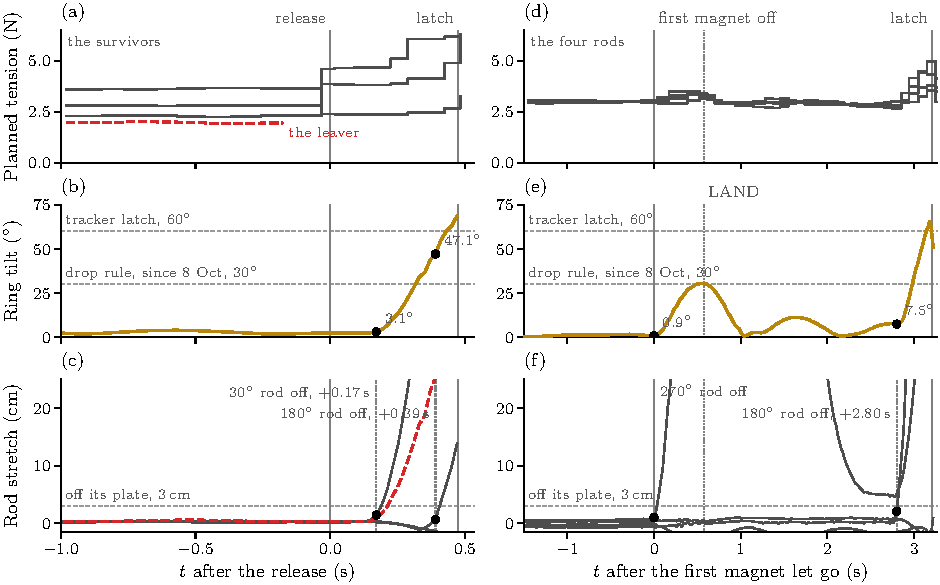
\includegraphics[width=\textwidth]{Images/magnet_anatomy.pdf}
\caption[How the ring was lost]{How the ring was lost on the rig on 7 October, twice, both with the rods planned at
45$^\circ$ (the panels print counter-clockwise azimuths: 30$^\circ$ is plate 11, 90$^\circ$ plate 9, 180$^\circ$ plate
6, 270$^\circ$ plate 3). Left, an announced release from plate 9 of a hover on plates 3, 6, 9 and 11 on the planner's
pull: (a) the planned tension per rod, with the survivors' step at the resize; (b) the ring's tilt; (c) each rod's
measured length over its own: 0.17\,s after the release the rod on plate 11 let go with no command, at 2.6$^\circ$ of
tilt, the rod on plate 6 followed, and the trackers latched the fleet at 60$^\circ$. Right, the circle on the measured
pull on the even ring: (d) the planned tensions, 3.0\,N each; (e) the tilt; (f) the rod on plate 3 let go with no
command at 0.9$^\circ$ of tilt and the ring recovered from 31$^\circ$; during the landing the rod on plate 6 let go and
the ring capsized.}
\label{fig:F11}
\end{figure}

All four releases of 8 October held the ring 5.3--6.8\,cm from its reference before the release, against 2.1\,cm
in the measured-pull hover of the day before: they ran the reference-shift integral, where the model integral, now
kept through a resize, is what L8 and L9 fly.

\subsubsection{The levers in the twin}
\label{sec:res_levers}

In the twin cell the rig's next hover release flies (plates 3, 7, 9 and 11, the magnet on plate 9 switched off
unannounced, the measured pull and the model integral), the planner hands the leaver's share to the three survivors in
one tick, as the statics of the even triangle say, and the tilt rise was 5.5--7.7$^\circ$ over three runs with the
release moved by 0.5\,s between them, only the first at the rig cell's timing (Figure~\ref{fig:detach}, Appendix~\ref{sec:app_secondary}).

\paragraph{The pull source on an unannounced release.} The frozen one-degree-of-freedom model (Section~\ref{sec:discussion})
predicts that on an unannounced release the measured pull, which follows the rod from its first samples, beats the
planner's pull, which flies the four-UAV shares until the resized plan arrives (a new prediction). In the twin cell
the prediction names (Figure~\ref{fig:F10b}), the measured rod pull kept the tilt rise to 5.5--7.7$^\circ$ where the
planner's pull let it reach 16.6--17.1$^\circ$; the means differ by 10.4$^\circ$ against the 4.4$^\circ$ the rule
requires, so the prediction is confirmed for this cell. The pair settles the sign, not the mechanism: the two arms do
not start from the same state, since on the planner's pull the ring hung 2.0$^\circ$ tilted at a steeper rod
elevation before the release. The announced half of the crossover, where the planned pull is predicted to win, has
not been flown.

\begin{figure}[htbp]
\centering
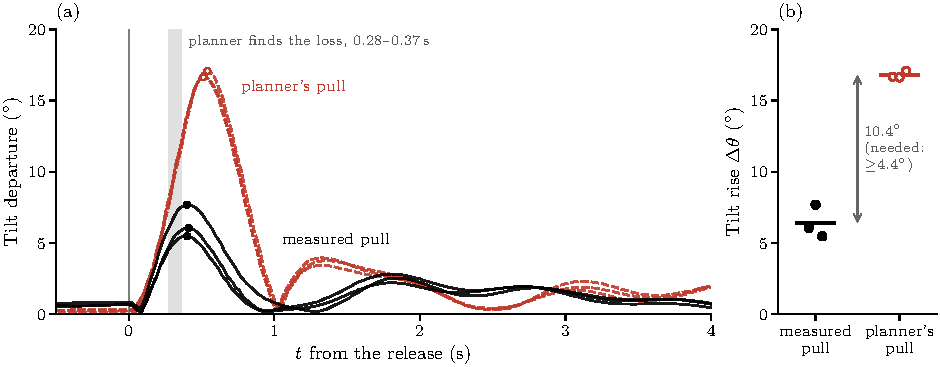
\includegraphics[width=\textwidth]{Images/crossover.pdf}
\caption[The pull source on an unannounced release]{An unannounced release in the twin, one cell: four UAVs
hover the ring at 1.0\,m from plates 3, 7, 9 and 11 and the magnet on plate 9 opens without telling the planner; the
model integral; three runs per pull source. (a) The ring's tilt departure against time, black with the survivors on
the measured rod pull, red on the planner's pull; marker: each run's tilt rise $\Delta\theta$; grey: the planner
finding the loss, 0.28--0.37\,s after the release. (b) $\Delta\theta$ per run and the arm means, 5.5--7.7$^\circ$
against 16.6--17.1$^\circ$: 10.4$^\circ$ apart against the 4.4$^\circ$ the frozen rule requires. The arms do not start
from the same state: on the planner's pull the ring hung 2.0$^\circ$ tilted before the release.}
\label{fig:F10b}
\end{figure}

\paragraph{The support margin.} The statics of Section~\ref{sec:reconfig} predict a larger transient for a smaller
margin, and the twin confirms it on the measured pull (Figure~\ref{fig:F12}b): moving the third survivor so that the
largest gap grows from 120 to 165$^\circ$ took the tilt rise from 5.5--7.7$^\circ$ at a 112\,mm margin to 7.8--9.1,
16.7--17.0 and 27.9--28.1$^\circ$ at 86, 58 and 29\,mm. Both pairs on rig plates resolve with the predicted sign (the second also with the drop
rule off) and no neighbouring pair the other way (Table~\ref{tab:T9}, Appendix~\ref{sec:app_levers}); at 29\,mm the ring came within
1.9--2.2$^\circ$ of the drop rule. With no margin (a 180$^\circ$
gap) three UAVs cannot hold the ring: with the drop rule off, the trackers' 60$^\circ$ latch disarmed the fleet in the
air 0.6\,s after the release, and on the default rules the planner's gap rule dropped the ring when it found the loss. At a 150$^\circ$ gap the planner's pull reached the drop rule in both runs and the ring was
dropped, which also confirms the pull-source prediction at that margin; with the measured pull every peak at gaps up
to 150$^\circ$ stayed under 30$^\circ$ (largest 16.9$^\circ$). The bar frozen as ``no run at gaps up to 150$^\circ$
reaches the drop line'' is therefore falsified as written, by the planner's pull. The twin has no magnet holding limit:
the curve speaks for the planner and the statics, not for a margin of safety on the rig.

\paragraph{What detecting the release buys.} On the planner's pull, detection decides the outcome: with detection off
the planner never resizes, and the tilt rise reached 28.2$^\circ$ in all three runs against 16.6--17.1$^\circ$ with it,
the tilt creeping to within 1.5--2.4$^\circ$ of the drop rule (confirmed, a new prediction). On the measured pull,
detection made no difference the rule could resolve at three runs (means 5.6 and 6.4$^\circ$, with the detection-on
arm's own range 2.2$^\circ$), as the pure model predicts. At landing what detection buys in this cell is the freed UAV's own landing: with detection off it never learns that it
left; on the three UAVs still on the ring the landing lean is unresolved on either pull source.

\paragraph{Carrying a circle with no event.} On the 60$^\circ$ circle with no release, the planner's pull tracked
better in the twin than the measured pull, 0.49--0.58 against 0.87--0.98\,cm mean path error (the even ring, two runs
each, 0.09\,cm over the frozen floor), but held height and tilt less evenly (height standard deviation 0.41--0.42
against 0.10\,cm). This is a replication of the earlier stack's order and not the rig's falsifier, which needs the
planned-pull 60$^\circ$ circle on the rig (K4).

\begin{figure}[htbp]
\centering
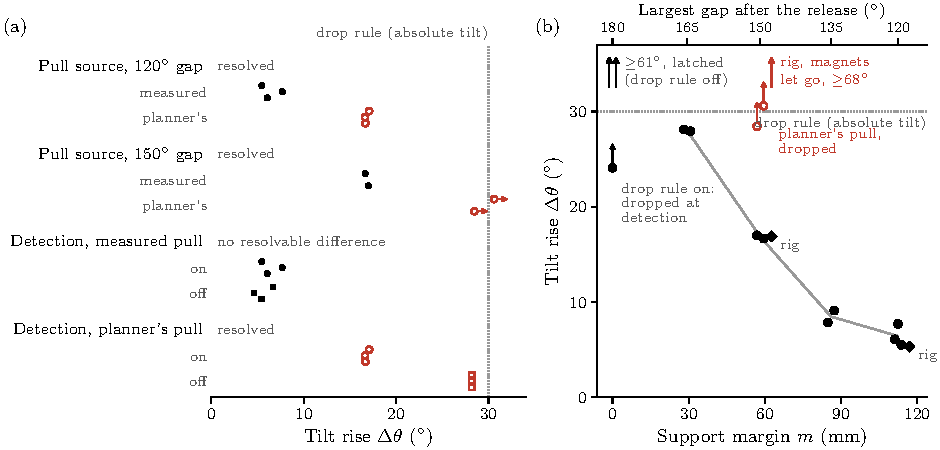
\includegraphics[width=\textwidth]{Images/levers.pdf}
\caption[The other levers]{The other levers in the twin: unannounced hover releases, the model integral, one marker per
run; arrow or triangle: a lower bound, cut where the ring was dropped or the fleet latched. (a) One-variable pairs: the
pull source with a 120$^\circ$ and a 150$^\circ$ gap, and detection on and off on each pull source (filled: measured
pull; hollow: the planner's pull), with each pair's verdict under the frozen rule. (b) $\Delta\theta$ against the
support margin $m = r\cos(g/2)$ of the largest gap $g$ left (top axis), on the measured pull: 5.5--7.7$^\circ$ at
112\,mm to 27.9--28.1$^\circ$ at 29\,mm; at zero margin the fleet latched with the drop rule off (arrows) and the gap
rule dropped the ring on the default rules (filled triangle); hollow triangles: the planner's pull at 58\,mm, dropped;
diamonds and red arrow: the rig's releases of 8 and 7 October. The twin has no magnet holding limit.}
\label{fig:F12}
\end{figure}

Appendix~\ref{sec:app_levers} gives every pair in one table with its frozen sign, its label and its verdict.

\subsubsection{The switch itself}
\label{sec:res_switch}

The resize is a switch between two optimal control problems of different size, and Table~\ref{tab:T10} measures it at
the first live solve of the smaller problem. No solve failed at any of 26 switches, 20 in the twin and 6 on the rig;
every first solve was as converged as the last solve before it, and on the rig the first solve took 24--28\,ms, though 2 of 66 solves in the next second passed the 60\,ms
budget. On the measured pull the survivors' throttle step is the release's, not the switch's (runs that never switch
read the same); on the planner's pull it is the planned share arriving. The gap to an offline solve run to convergence
is not computed.

% generated by tools/thesis_freeze_tables.py; run ids in docs/figures/PROVENANCE.md
\begin{table}[htbp]
  \centering
  \footnotesize
  \setlength{\tabcolsep}{3pt}
  \caption[The switch itself]{The switch itself (T10): the planner's first solve of the smaller problem when a UAV
  leaves, and the second after it; $n$ switches. Status: the solver's status at the first solve, then the failed solves
  in the second after it. KKT residual: stationarity and dynamics at the first solve, the largest in the row. Solve time, rig only: the first solve and
  the longest in the second after it (60\,ms budget). Throttle step: the survivors' largest throttle
  departure in the 0.3\,s after the switch, over their hover throttle; in brackets, the same statistic at the planner
  ticks of the steady hover before.}
  \label{tab:T10}
  \begin{tabularx}{\textwidth}{>{\raggedright\arraybackslash}p{1.6cm}>{\raggedright\arraybackslash}Xcccc}
    \toprule
    Switch & Data ($n$) & Status; failed & KKT residual (stat / eq) & Solve time (ms) & Throttle step (\%) \\
    \midrule
    Leave, announced & Rig, planner's pull$^a$ (2) & 0; 0 of 22 & $1.1\times10^{-3}$ / $1.1\times10^{-7}$ & 24--28; 58--60 & 12.6--15.8 (1.2--3.9) \\
     & Rig, measured pull (1) & 0; 0 of 11 & $6.5\times10^{-5}$ / $2.4\times10^{-8}$ & 26; 35 & 15.9 (7.3) \\
    Leave, unannounced & Twin, measured pull, gap 120--165$^\circ$ (13) & 0; 0 of 130 & $3.8\times10^{-4}$ / $2.3\times10^{-7}$ & -- & 1.9--5.7 (0.4--0.9) \\
     & Twin, measured pull, gap 180$^\circ$$^b$ (2) & 0; 0 of 21 & $3.9\times10^{-4}$ / $1.7\times10^{-8}$ & -- & 11.5--12.1 (0.4--0.5) \\
     & Twin, planner's pull, gap 120--150$^\circ$$^c$ (5) & 0; 0 of 34 & $9.9\times10^{-5}$ / $2.4\times10^{-8}$ & -- & 11.4--16.8 (0.4--0.5) \\
     & Rig, measured pull (3) & 0; 0 of 33 & $3.3\times10^{-4}$ / $2.9\times10^{-7}$ & 25--26; 32--62 & 9.2--13.3 (6.8--9.4) \\
    Join (hand-over) & [the join code tree] & [\dots] & [\dots] & [\dots] & [\dots] \\
    \bottomrule
    \multicolumn{6}{>{\raggedright\arraybackslash}p{\dimexpr\textwidth-2\tabcolsep}}{\footnotesize $^a$\,Rods planned at
    45$^\circ$; in one of the two flights two magnets then let go and the ring capsized (Figure~\ref{fig:F11}).
    $^b$\,No margin, the drop rule off: the fleet latched 0.4\,s after the switch. $^c$\,In 2 of 5 runs the trackers'
    30$^\circ$ rule dropped the ring 0.2\,s after the switch; the window ends there.} \\
  \end{tabularx}
\end{table}


\subsubsection{The freed UAV}
\label{sec:res_freed}

On 8 October the freed UAV's own landing did not finish on the rig: it floated above its rest until the fleet's disarm
dropped it about 0.3\,m. Its reference is now pressed down to its own rest, and once there it is disarmed alone
(Figure~\ref{fig:departed_landing}, Appendix~\ref{sec:app_secondary}). On the freeze code tree it was disarmed alone
0.27--0.43\,s after it first reached its rest, within 2\,mm of it and before the fleet landed, in every hover and circle
release (five runs); on the rig the rule has so far acted only in the drop of 15 October (L11).

\subsubsection{Losing a second carrier: the drop}
\label{sec:res_drop}

A loss that leaves fewer than three carriers, or a ring tilted past 30$^\circ$, drops the ring
(Section~\ref{sec:safety}). On the freeze code tree in the twin, a second loss after a first, and a first release that
leaves a 240$^\circ$ gap, were each flown twice: the ring was dropped 0.22--0.23\,s after the loss, no UAV tilted past
13.6$^\circ$ or climbed more than 0.18\,m, and every UAV was down (below 0.15\,m) within 8.5--8.9\,s and disarmed
0.10--0.11\,m above the floor, with no fault. Which rule fires first, the planner's gap rule or the trackers' tilt request, is a race,
and the margin to the trackers' 60$^\circ$ latch is thin, 0.06--0.12\,s in the twin. On the rig the rule fired once, on 15 October (L11, above), and landed every carrier.

\paragraph{Answer to RQ2.} What sets the ring's transient when a carrier leaves is, first, geometry: in the twin the tilt
rise grew as the support margin the leaver leaves behind shrank, from 5.5--7.7$^\circ$ at 112\,mm to
27.9--28.1$^\circ$ at 29\,mm, and with no margin three UAVs cannot hold the ring. Second, the pull source the survivors
fly on: in the two twin hover cells flown (120 and 150$^\circ$ gaps) the tilt rise was smaller on the measured pull than
on the planner's pull, a sign and not yet a mechanism, and on the planner's pull detecting the release held the rise at
17$^\circ$ where without it the tilt crept to within 1.5--2.4$^\circ$ of the drop rule.
The resize itself is a clean switch: no solve failed at 26 switches. On the rig three UAVs carried the ring on through
five of six commanded releases with tilt rises of 5.3--16.9$^\circ$. What loses a ring is a magnet letting go: all four
rings lost on the rig began that way, twice after the rods were planned at 60$^\circ$, and the drop rule, on in every
mode since 14 October, landed the fleet when it happened again on 15 October.
